\chapter{Transformers}\label{ch_transformers}
\chapterauthor{Jeff Yoshimi}

% TODO: Title LLMs and Transformers?
% Encoders, decoders, masking, other cases.  For example, we can feed a transformer network the first halves of hundreds of movie scripts and train it to produce the second halves of those scripts, or we can train it to predict what the first summary paragraph of a Wikipedia article is based on the main body of the article.
% Mention fine tuning and other things built  on top of the underlying model.  See Kauf and Ivanova 2023
% Add glossary items for llm, transformer, auto-regression , token, context window, etc.

In 2020 the power of recurrent networks reached another milestone with the introduction of Open AI's model, GPT-3 \cite{brown2020language, floridi2020gpt}, and with the introduction of ChatGPT in 2022 neural networks and AI broadly entered another stage of historical development (see chapter \extref{ch_history}). For example, they have changed the way authorship and education will work, because they can write arguably professional-level papers and artworks. In this chapter we cover large language models (LLM's) and transformers and associated technologies, which are at the basis of ChatGPT.

% Glossary on token and ref to nlp
% Input-to-output recursion and how this in a way gets us the recurrent link this evolved from
A \textbf{large language model} is a class of neural network models which can generate text responses to text inputs by repeatedly predicting the next word in a sequence. They often use an architecture called the \textbf{transformer architecture}, which is a many-layered feed-forward network with special mechanisms for leaning relationships between tokens (see chapter \extref{ch_word_embeddings}) in a context.  This architecture builds on many of the insights of past chapters. As we will see, they can be trained using ``auto-regression'', which converts widely available text data into the input-target format of a training dataset (chapter \extref{ch_data_science}). Earlier efforts at text generation and natural language processing used supervised recurrent networks (chapter \extref{ch_supervised_recurrent}), which are in various ways limited. By using feed-forward networks to accomplish the same task, all the accumulated insights of decades of research could be leveraged. A transformer is in fact just a really complex feed-forward supervised network running a form of backprop (chapters \extref{ch_supervised}, \extref{ch_lms_backprop}). It also draws on the lesson of the deep learning revolution (section \extref{deep_revolution}), using many layered ``deep'' networks (chapter \extref{ch_deep_nets}) that develop complex representations and can be trained on large datasets using highly optimized parallel hardware.

% But is it a rep? It is inside the network not outside it.
%The key innovation with transformers is, in a sense, a special kind feature representation (compare the discussion of feature engineering in chapter \extref{ch_data_science}).  Tokens are converted into vectors using word embeddings, and sequences of these vectors are all fed into the network and compared. This gives the network a sense of context.

In this chapter we cover the basic idea of the architecture, and then consider how it can be used in cognitive science, to identify learned internal representations that are psychologically meaningful. Changes in this area is rapid, and the relevance of these areas to cognitive science is only now being studied, so updates to this chapter are expected.

\section{Autoregression}

First let's see how the training data work. Recall from chapter \extref{ch_data_science} that a training dataset consists of inputs and targets, and is also called a labeled dataset. This kind of labeled data can be hard to get, as we saw.  We might have lots of pictures of people but not know the names or identities of the people in the pictures, or lots of pictures of cats and dogs but not whether a given picture is a cat or dog.  The method of  \textbf{auto-regression} provides a way to take \emph{any piece of text} and convert it into a training data set. The trick is to take a set of tokens in a text as input, and then to use the next token as the target, or label.  Any text will do! For example, consider this block of text adapted from the Wikipedia page for UC Merced:

\begin{quote}
The University of California, Merced is a public land-grant research university in Merced, California. It is one of the ten campuses in the University of California (UC) system. Established in 2005, Merced is the newest campus within the UC system.
\end{quote}

From this can create a bunch of training examples, a bunch of input / target pairs. We might use ``The University of California" as an input, and then ``Merced'' as a target. Or we can use ``Merced is a public land-grant'' as an input, and then ``research'' as a target.  We simply associate each token in the input with a vector using a word embedding, and the target with an embedding, and we can build a table of input-target vector pairs, which we can use to train a feed-forward neural network.  For a sense of the idea, see figure \ref{contextWindow}. 

% TODO: A picture might still be nice here
  
\section{How Text is Generated from a Feed-forward Network}

% Recursion trick. Inputs include past outputs.

Let's see in more detail how text can be generated by an LLM using a feed-forward network. Suppose we want to ask a network ``hello how are you?'' In a recurrent network (chapter \extref{ch_supervised_recurrent}), a vector representation of each token in the sequence would be presented separately: ``hello'', ``how'', ``are'', ``you'', and ``?''.  In a transformer, by contrast, we arrange these vector embeddings into a single vector and present them all at once to the network. That is, the input to the network is the whole sentence $\{$``hello'', ``how'', ``are'', ``you'', ``?''$\}$. Let's initially not worry about the vector embeddings, and just see the general idea, as shown in figure \ref{gptRecursedInputs}. Notice that the initial prompt is the initial input, but then the prompt \emph{and} the first word of the response are used as the next input, and this process can be repeated until a response is written out.\footnote{How does it know when to stop? This is based on a separate system trained using reinforcement learning and policy gradient descent.}
  
% More rounds might be needed to clarify this

\begin{figure}[h]
\centering
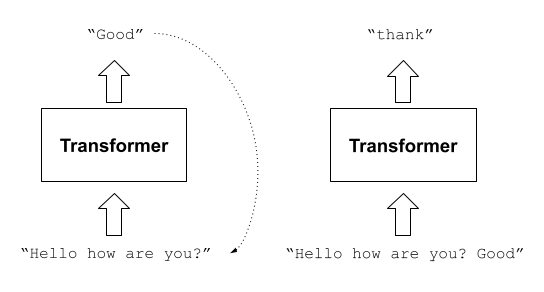
\includegraphics[scale=.7]{./images/gptRecursedInputs.png}
\caption[Jeff Yoshimi]{A schematic view of how ``conversations'' are generated from a feed-forward network in systems like GPT. The output from one moment is added to the end of the input, and the new input is then fed in. The process is repeated to generate a full response.}
\label{gptRecursedInputs}
\end{figure}

% Glossary
Now let's add the vector embeddings. A feed-forward network takes a fixed size input.  In an LLM this is called its \textbf{context window}. GPT-3 has a context window of about 2000 tokens or about 6 pages of text, and early versions of GPT-4 had context windows of 32,000 tokens or about 72 pages of text.  As you say more things to the system, the inputs will include all your past prompts and all of its own responses in one big input.  Of course, initial prompts don't use that many tokens, so the extra space is padded or ignored in some way, for example with zero vectors. With this in mind, let's consider what some of the training data used to train a network to respond to ``hello how are you?" with ``fine thank you'' might look, using a three-dimensional word embedding. See figure \ref{contextWindow}. 

\begin{figure}[h]
\centering
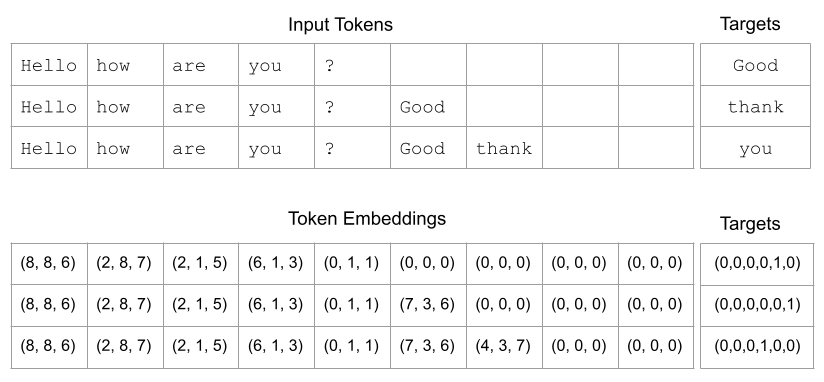
\includegraphics[scale=.45]{./images/contextWindow.png}
\caption[Jeff Yoshimi]{What some training data might look like for the example in figure \ref{gptRecursedInputs}. The top row panel shows the tokens in three training examples and the bottom row shows the corresponding token embeddings.  It should be clear that the bottom panel shows inputs that can actually be fed into a neural network, in this case, a network with 27 input nodes. Note that the targets are one-hot encoded, because these networks are actually classifiers. They have one ``node'' for each token in this small vocabulary. In this case, there are 7 nodes for the 7 tokens: ``Hello'', ``how'', ``are'', ''you'', ``?'', "Good'', ``thank''.  }
\label{contextWindow}
\end{figure}

% Softmax ref and RL ref.  In RL add mention of policy gradients and then a ref to gradient descent!
Note that the targets are one-hot encoded over the entire vocabulary. The output layer of a model like this is something like a probability distribution over all possible tokens (7 in this example, but over 50,000 in GPT). Thus the output is a a probability distribution over all the words of the English language. The output layer of the network lights up most for words that would normally come after the current input, which includes all prompts and responses so far in the context window. 

Notice that since the target data are binary one-hot encoded labels, the task given this network is actually a classification task (section \extref{classificationRegression}). The network is classifying context window inputs into categories corresponding to what the next token should be.  For any context window input, the output is a probability over next tokens, and one of the most probable next tokens is selected. From this probability distribution a relatively probable token is selected and added to the current context window as the next input. This process is repeated until the network is finished responding.

\section{Learn to speak Internetese}

In section \extref{languageModelsRecurrent} we saw how language models trained on example text would learn to speak in a certain way that reflects the statistical properties of the training data. A network trained on Shakespeare would start to speak fake Shakespeare, fake math was generated, etc. 
Large language models using transformers do the same thing, they just do it much better. They use larger datasets (hence ``large'' being added in front of ``language model''), and they use a feed-forward transformer architecture that, as of this writing, outperforms recurrent architectures. 

% TODO Check
The training set for GPT is not all of Shakespeare, or a bunch of math papers, but a much larger dataset that encompasses both of those and much, much more (see figure \ref{gptDatasets}).  In particular, it includes all of Wikipedia, a few compilations of books, and a web-scraped archive of a large subset of the \emph{entire internet}, called common crawl (\url{https://en.wikipedia.org/wiki/Common_Crawl}.) If you've ever written anything online, there is a decent chance it is part of the training data that was used! It is an absolutely massive dataset. Using auto-regression the whole dataset can be converted into a labeled dataset, just using this freely available text.  Also the network used to process it is massive (see figure \ref{gptParams}). 

Since all of Shakespeare is on the internet, and discussions of every topic of human endeavor from physics to history, and plenty of gossip and randomness about popular culture and everything else, it can talk about all of these things.  It can statistically generalize from its training data, which in this case is primarily a large part of the internet. Thus, in a sense, it learns to speak ``internetese''.  (Also note that common crawl and GPT-4 are regularly updated, so it stays up to date within a year-or-two). 
% Reference above

% TODO: This and the one below
\begin{figure}[h]
\centering
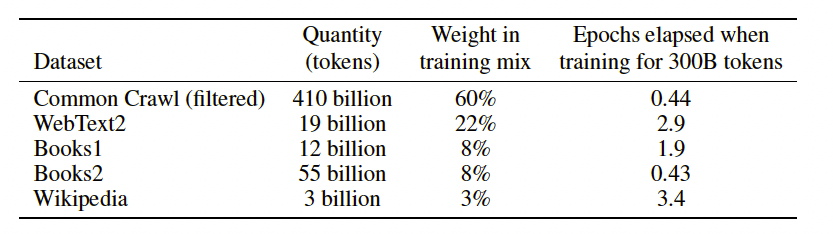
\includegraphics[scale=.4]{./images/gptDatasets}
\caption[GPT Technical report. Todo]{The datasets used to train GPT-3. Mostly internet, but lots of books and all of Wikipedia too. }
\label{gptDatasets}
\end{figure}

% Turing test more citations
The results are impressive. The texts it produces are no longer obviously fake in the way the examples from section \extref{languageModelsRecurrent} were. In fact, in some cases it arguably passes the Turing Test, a long-standing test for artificial general intelligence, answering questions and producing convincing  text in response to prompts.\footnote{\url{https://plato.stanford.edu/entries/turing-test/}. Whether GPT really passes the test is a matter of ongoing controversy.} For example, when asked to write an article with the title ``United Methodists Agree to Historic Split: Those who oppose gay marriage will form their own denomination'', it produced the following:
\begin{quote}
After two days of intense debate, the United Methodist Church has agreed to a historic split - one that is expected to end in the creation of a new denomination, one that will be ``theologically and socially conservative,'' according to The Washington Post. The majority of delegates attending the church's annual General Conference in May voted to strengthen a ban on the ordination of LGBTQ clergy and to write new rules that will "discipline" clergy who officiate at same-sex weddings. But those who opposed these measures have a new plan: They say they will form a separate denomination by 2020, calling their church the Christian Methodist denomination...
\end{quote}
Most people can't tell that this was written by a computer.  This kind of text generation was big news back in 2020, but of course, it's run-of-the-mill now that we are all familiar with GPT.

\section{The Transformer Architecture}\label{transformers}

So, how does GPT work? How does it achieve all this? Much of its power rests on its ability to use a deep feed-forward network, lots of training data, and a large context window (thousands or millions of tokens rather than just 9 as in the example above; think of a Simbrain network with \emph{millions} of input nodes). This is key: it can process everything in a large context of discussion.  And it has many layers--in recent versions more than 100--allowing it to develop highly complex representations.
% TODO: I think it is d_head * num_heads

The transformer architecture \cite{vaswani2017attention} contains layers or ``blocks'' which are specialized to process the large context windows that are fed to the network as input. With training they learn to find long-range dependencies between different parts of a context window (which includes an original prompt, its own response to that prompt, etc.; it includes the \emph{entire exchange} you've had with GPT up to the current point, so long as it fits in the context window). Each block combines  a ``self-attention'' layer with a traditional linear layer and several other mechanisms (see figure \ref{transformerBlock}). The self-attention layer is where the magic happens.  One part of this layer compares each token in the context window to every other token in the window. In our simple example, ``hello'' is compared to ``hello'', ``how'', ``are'', and ``you'', and this comparison is used to create a representation of the sentence that reflects dependencies between the words. All words are compared to each other in the context window, so that no matter how far apart they are, they can still influence each other. The self-attention mechanism learns what relations between words in a context window are important; in a sense it learns what to focus on (hence ``self attention''). This ability to find meaningful relationships within an input sequence is part of why transformers are relevant to cognitive science, as we will see.

\begin{figure}[h]
\centering
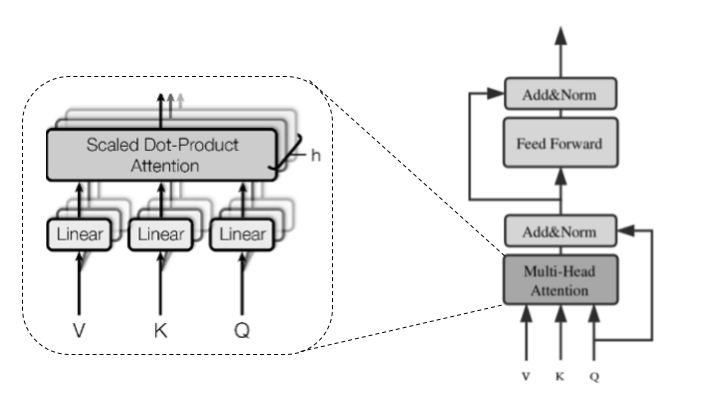
\includegraphics[scale=.4]{./images/transformerBlock.png}
\caption[Jeff Yoshimi modification of Todo.]{One layer of a transformer architecture, which is also called a ``block''. }
\label{transformerBlock}
\end{figure}
% More on normalizing. See neuralnets.txt.  Also need a picture to show that input and output are same-sized.

The details of what occurs in a block are not developed in detail here though we are planning to expand the discussion in future versions of this chapter. However, here is a rough sketch of what happens. Input tokens in a context window are vector embedded (via the links labeled ``linear'' at the bottom) and these vectors are matrix multiplied by shared weight matrices labeled $v$, $k$, and $q$ to produce value, key, and query vectors for each input token (the $v$, $k$ and $q$ matrices are like the weights that are trained via backprop). The key and query vectors are matrix multiplied in all combinations to create a matrix of self attention scores. This captures relationships between tokens in a context window. These scores are multiplied by the value vectors. This entire process happens once for each head. The outputs of all the heads are squashed back together and normalized, and put through a standard feed-forward network of the kind we've been talking about throughout the book. The output of the block is a set of vectors that has the same shape as the input vectors.  For example, in the example in figure \ref{contextWindow} the input would be 9 vectors with 3 components each, and the output would be too. For a nice visualization that is vaguely in the Simbrain style, see \url{https://bbycroft.net/llm}.

Within each block all the mechanisms above are separated out into multiple ``heads''. As a result, the network can learn \emph{multiple} ways to compare words in the sentence to each other, a bit like how a convolutional network (section \extref{convolutionalLayer}) develops \emph{multiple} filters to analyze an image.  The results of these different attention heads are combined and as a result each layer of a transformer network involves a sophisticated representation of the sentence that represents multiple types of inter-word dependency.

% Ref to some of the interpretation stuff. also ref to internal reps and yamins
Now we take a lesson from deep networks, and stack many of these transformer blocks on top of each other, to produce increasingly sophisticated representations.  Recall that with deep networks for vision, we get features, features of features, features of these features, etc. whose activations match neural response properties of different layers of the human visual system. This builds on the old idea of the \emph{Pandemonium} model (section \extref{cog_rev}), which involved (at successive layers): edge detectors, detectors for combinations of edges, detectors for combinations of these combinations (e.g. fragments of letters), and ultimately letter detectors. In a similar way, the successive layers of a transformer model of language correspond to increasingly complex features of the input stream, including syntactic categories, semantic properties, and far more complex features as well. We return to this topic at the end of the chapter, but note that understanding the nature of these representations is still in its infancy. The transformer model was not built to help cognitive science, after all, but to support NLP engineering tasks. Nonetheless, the results are so compelling that they are of interest to cognitive scientists.

There are also a number of other tricks used to represent this sentence in a useful way that facilitates parallel processing and improve on recurrent networks.\footnote{In particular positional encodings, a special form of vector that can be added to a word embedding that tags it for its location in a sequence. Since words are intrinsically tagged with their position, they can be processed in parallel, which allows the architecture to run on fast parallel hardware. A kind of feature engineering trick (chapter \extref{ch_data_science}).  }

Some of the parameters for GPT-3 are shown in figure \ref{gptParams}. Some are familiar, like learning rate. Others describe number of layers. Others the number of heads. All are large and much larger with GPT-4.

% Say more about this. Be sure hyperparams are defined.  Would be good to make sure each hyperparam is explained and referenced somewhere. Check that d_model is embedding dimension and explain that.
\begin{figure}[h]
\centering
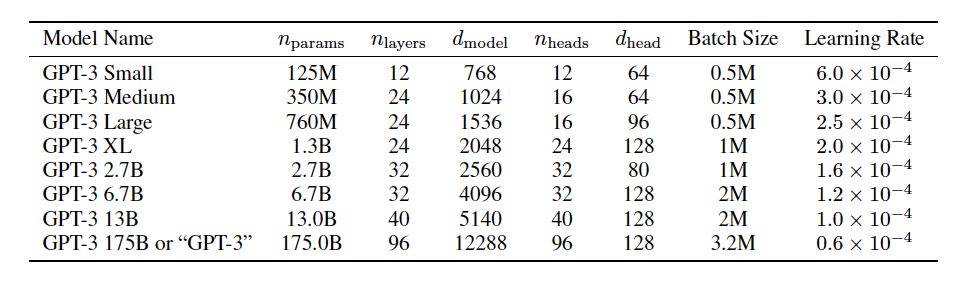
\includegraphics[scale=.4]{./images/gpt3_params.png}
\caption[GPT Technical report. Todo]{Some of the hyper-parameters used in training different versions of GPT-3. Some of these are familiar to us, others are new. Notice the number of parameters, which are primarily weights and biases.  Billions, and GPT-4 is approaching 2 trillion parameters.  That is a lot of weights and biases.  Our xor 2-2-1 network had 3 biases and 6 weights, 9 parameters.  A standard convolutional neural networks might have millions of parameters. So this is just massively larger. }
\label{gptParams}
\end{figure}

\section{Bert}\label{sect_bert}

Transformer networks have been extremely successful. They have also revolutionized natural language processing, via the BERT language model, which is making an impact in the cognitive sciences, especially in the computational study of language. In a paper co-authored by Jay McClelland  \cite{mcclelland2020placing} (a member of the original PDP group at UCSD; see section \extref{first_resurgence}), the following example is used to illustrate the point:
\begin{quote}
John put some beer in a cooler and went out with his friends to play volleyball. Soon after he left, someone took the beer out of the cooler. John and his friends were thirsty after the game, and went back to his place for some beers. When John opened the cooler, he discovered that the beer was \rule{1cm}{0.15mm}.
\end{quote}
The reader expects the word ``gone'' next, but if ``took the beer'' is replaced with ``took the ice'' the reader expects something like ``warm''. But the first part of the sentence is too far apart from the last part for an unrolled backprop through time network to pick up the relationship.  Transformer networks like BERT overcome this problem.

The big questions are: how exactly does BERT do this, and whatever it does, is it relevant to human language processing?  This creates a fascinating twist on our earlier discussion of types of neural network research (section \extref{typesOfResearch}). Recall that neural networks are sometimes used for engineering, sometimes for science, but that there is a feedback between these categories of research. For example, deep convolutional networks originated in scientific studies of visual processing, got refined and used for pattern recognition tasks in engineering, and the resulting deep networks were so powerful that they were then taken back into science  to describe (for example) the human visual system.
Additionally, the training task for BERT differs from other contemporary language models; BERT uses ``masked language modeling'' (MLM) instead of traditional next word prediction.\footnote{See \cite{devlin2018bert} for a detailed explanation.} Instead of modeling language as a left-to-right stream of words, where the model predicts the next word based on the previous context, BERT instead masks a token in the middle of the sentence, and predicts it based on the surrounding sentential context. This is advantageous over unidirectional left-to-right and concatenated left-to-right and right-to-left models, since it creates a truly bidirectional representation where the left and right contexts are joined together.

Here we see a variant on that pattern. In this case, recurrent neural networks (with their own long history spanning cognitive science and engineering) weren't performing well enough, so engineers created these new transformer architectures, mainly to tackle engineering issues like vanishing gradients and parallelization.  They used the intuitive concept of attention, but it was all engineering. BERT came out of Google and fit their engineering needs. Psychologists and linguists then realized  BERT was doing better at analyzing language than other models in linguistics, so they started to treat it as an object of scientific interest in its own right. This gave rise to a new field called ``BERTology''. In a paper titled ``A Primer in BERTology: What We Know About How BERT Works'' \cite{rogers2020primer}, a ``survey of over 150 studies of the popular BERT model'',  the authors explain:
\begin{quote}
Although it is clear that BERT works remarkably well, it is less clear why, which limits further hypothesis-driven improvement of the architecture. Unlike CNNs, the Transformers have little cognitive motivation, and the size of these models limits our ability to experiment with pre-training and perform ablation studies. This explains a large number of studies over the past year that attempted to understand the reasons behind BERT’s performance. In this paper, we provide an overview of what has been learned to date, highlighting the questions that are still unresolved.
\end{quote}
This is a strange situation. Engineers built something and then scientists created a science to understand it!  

Clearly there is a need for further study from connectionist and computational neuroscience standpoints (BERTologists are mainly computational linguists).  These networks develop complex internal representations using neural networks, which are brain like, and perform at amazingly human levels, as we'll now see.

% One shot learning etc.

% TODO: More on applications to cog-sci
% Ethics discussions? An old note: Some philosophical analysis of the promise and potential dangers of this technology are in \cite{floridi2020gpt}.